
\documentclass{beamer}
\usetheme{Pittsburgh}
\usecolortheme{spruce}

% for themes, etc.
\mode<presentation>
{ \usetheme{boxes} }

\usepackage{times}  % fonts are up to you
\usepackage{graphicx}
\usepackage{algorithm}
\usepackage{algorithmic}
\renewcommand{\algorithmicrequire}{\alert{Input:}}
\renewcommand{\algorithmicensure}{\alert{Output:}}

\setbeamertemplate{footline}[frame number]

% these will be used later in the title page
\title{Advanced Encryption Standard (AES)}
\author{ Lucas Zewen Ye \\ lucas.zw.ye@outlook.com }
\date{\today}

\AtBeginSection[]
{
\begin{frame}<beamer> 
\frametitle{Outline} % make a frame titled "Outline"
\setcounter{page}{0}	%setcounter似乎对beamer无效
\tableofcontents[currentsection]  % show TOC and highlight current section
\end{frame}
}


\begin{document}
% this prints title, author etc. info from above
\maketitle

\section{Polynomial in Finite Field}
\begin{frame}{Polynomial}
	$f(x) = a_n x^n + a_{n-1} x^{n-1} + ... + a_1x+a_0 = \sum_{i=0}^n a_i x^i$
	$g(x) = \sum_{i=0}^n b_i x^i$

	$f(x) + g(x) = \sum_{i=0}^n (a_i+b_i) x^i$

	$f(x) \times g(x) = \sum_{i=0}^{2n} c_i x^i, c_i = a_0b_i + a_1b_{i-1} + ... + a_ib_0$
\end{frame}

\begin{frame}{Finite Field $GF(p)$}
	A finite field is a finite set that multiplication, addition, subtraction and division are defined and satisfy the rules of arithmetic.

	Given a \alert{prime} $p$, the finite field $GF(p)$ is made up of $0, 1, 2, ..., p-1$ (totally $p$ numbers).
\end{frame}

\begin{frame}{Polynomial in Finite Field $GF(p^n)$}
	$f(x) = a_{n-1} x^{n-1} + ... + a_1x+a_0 = \sum_{i=0}^{n-1} a_i x^i, a_i \in {0,1,...,p-1}, i<n$

	if p = 3, n = 2, there are $3^2 = 9$ polynomials in $GF(p^n)$:
	$0, 1, 2, x, x + 1, x + 2, 2x, 2x + 1, 2x + 2$
\end{frame}

\begin{frame}{Irreducible Polynomial}
	$f(x) = x^6 + x^4 + x^2 +x +1, g(x) = x^7 +x +1, f(x),g(x) \in GF(2^8)$

	$f(x) \times g(x) = x^{13} + x^{11} + x^9 + x^8+ x^6 + x^5 + x^4 +x^3 + 1 \notin GF(2^8)$

	Solution: use \alert{Irreducible Polynomial} to reduce the result
	$m(x) = x^8+x^4+x^3+x+1$

	$f(x) \times g(x) \bmod m(x) = x^7+x^6+1$
\end{frame}


\begin{frame}{Arithmetic in $GF(2^8)$}
	$f(x) = x^6 + x^4+x^2+x+1 (binary: 01010111, hex: 0x57)$

	$g(x) = x^7 +x +1(binary: 10000011, hex(0x83))$

	$f(x) + g(x) = x^7 + x^6 + x^4 + x^2 (binary: 11010100, hex: 0xd4)$

	$0x57 \oplus 0x83 = 0xd4$

	Addition and Subtraction are equivalent to \alert{XOR}
\end{frame}

\begin{frame}{Arithmetic in $GF(2^8)$}
	$x^8 \bmod m(x) = m(x) - x^8$

	$f(x) = a_7 x^7 + ... + a_1x+a_0$

	$x \times f(x) = a_{7} x^{8} + ... + a_1x^2+a_0x \bmod m(x)$

	if $a_7 = 0$, $x \times f(x) =a_6x^7 +...+ a_1x^2+a_0x$

	else, $x \times f(x) =x^8 + a_6x^7 + ...+a_1x^2+a_0x = m(x) - x^8 + a_6x^7 +...+ a_1x^2+a_0x$

	In total,
	$$ x\times f(x)=\left\{
		\begin{aligned}
			(b_6b_5b_4b_3b_2b_1b_00), b_7                      & = 0 \\
			(b_6b_5b_4b_3b_2b_1b_00) \oplus bin(m(x)-x^8), b_7 & = 1
		\end{aligned}
		\right.
	$$
\end{frame}

\section{The Detail of AES}
\begin{frame}{Introduction}
	All the operations of AES are in finite field $GF(2^8)$

	The key length of AES can be 128 bit, 192 bit and 256 bit, with different round of encryption and decryption.
	\begin{table}[]
		\begin{tabular}{|l|l|l|l|}
			\hline
			Key Size(bit)     & 128 & 192 & 256 \\ \hline
			Plaintxt Size     & 128 & 128 & 128 \\ \hline
			Number of Rounds  & 10  & 12  & 14  \\ \hline
			Round Key Size    & 128 & 128 & 128 \\ \hline
			Expanded Key Size & 176 & 208 & 240 \\ \hline
		\end{tabular}
	\end{table}
\end{frame}

\begin{frame}{AES Structure}
	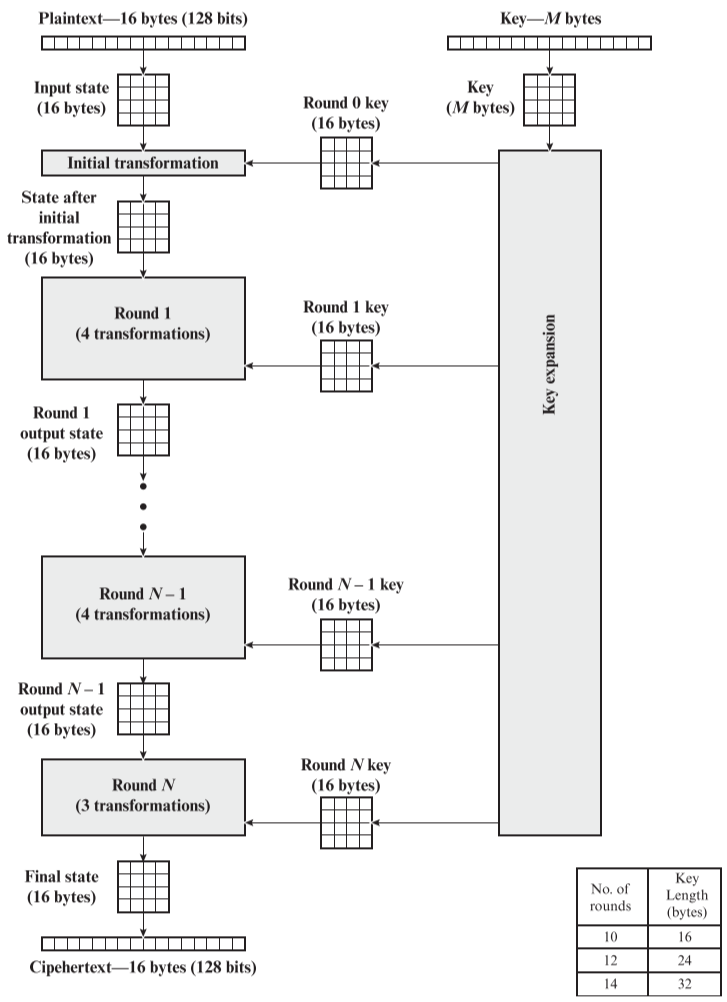
\includegraphics[width=2.3in]{fig/structrue.png}
\end{frame}

\begin{frame}{AES Structure}
	4 transformations:
	\begin{itemize}
		\item Substitute Bytes:
		      Uses an S-box to perform a byte-by-byte substitution of the block.
		\item ShiftRows: A simple permutation.
		\item MixColumns: A substitution that makes use of arithmetic over $GF(2^8)$.
		\item AddRoundKey: A simple bitwise XOR of the current block with a portion of the expanded key.
	\end{itemize}
\end{frame}

\begin{frame}{Substitute Bytes}
	S-box and Inverse S-box: 16 $\times$ 16 lookup table

	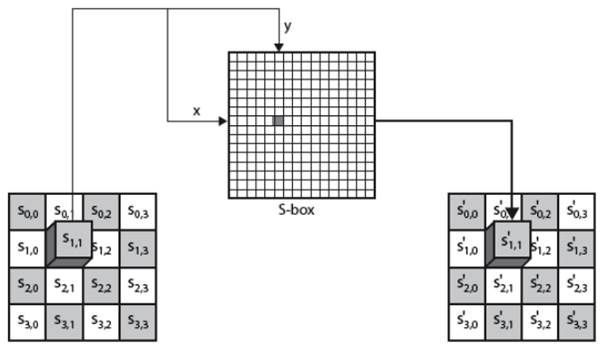
\includegraphics[width=4.3in]{fig/clip_image006.jpg}
\end{frame}

\begin{frame}{ShiftRows}
	\begin{itemize}
		\item 1st row is unchanged

		\item 2nd row does 1 byte circular shift to left

		\item 3rd row does 2 byte circular shift to left

		\item 4th row does 3 byte circular shift to left
	\end{itemize}

	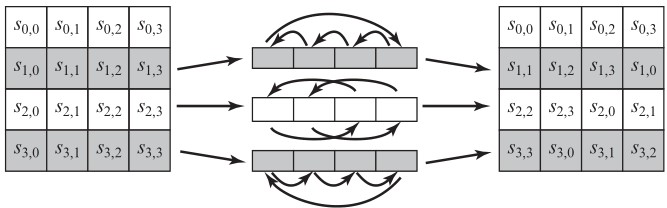
\includegraphics[width=4.0in]{fig/clip_image008.jpg}
\end{frame}

\begin{frame}{MixColumns}
	Multiplication with a matrix.
	\centering
	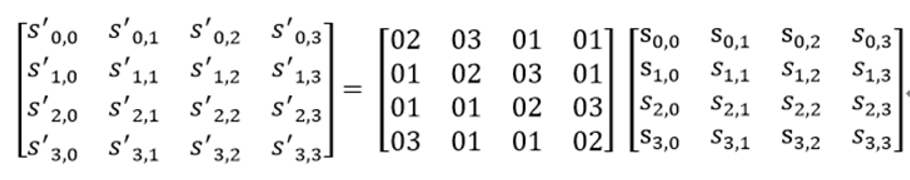
\includegraphics[width=4.5in]{fig/clip_image010.png}

	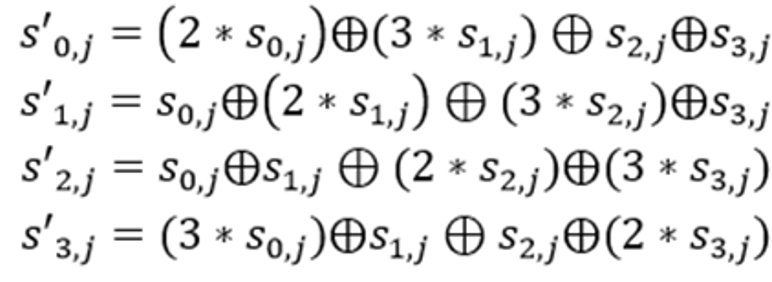
\includegraphics[width=2.5in]{fig/clip_image012.png}

	% 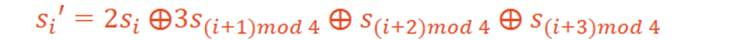
\includegraphics[width=4.0in]{fig/clip_image014.jpg}

	% 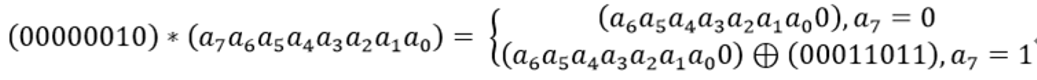
\includegraphics[width=4.0in]{fig/clip_image016.png}

	% 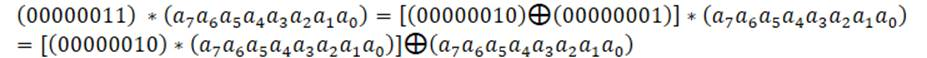
\includegraphics[width=4.0in]{fig/clip_image018.jpg}
\end{frame}

\begin{frame}{Add RoundKey}
	\centering
	XOR operation.
	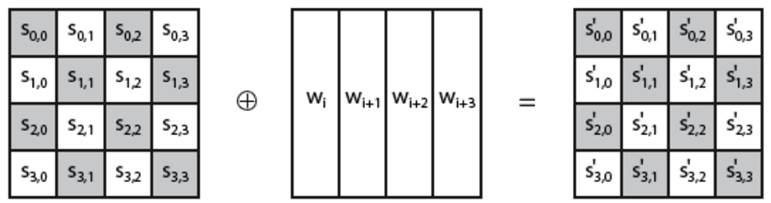
\includegraphics[width=4.5in]{fig/clip_image004.jpg}
\end{frame}

\begin{frame}{Single Round AES}
	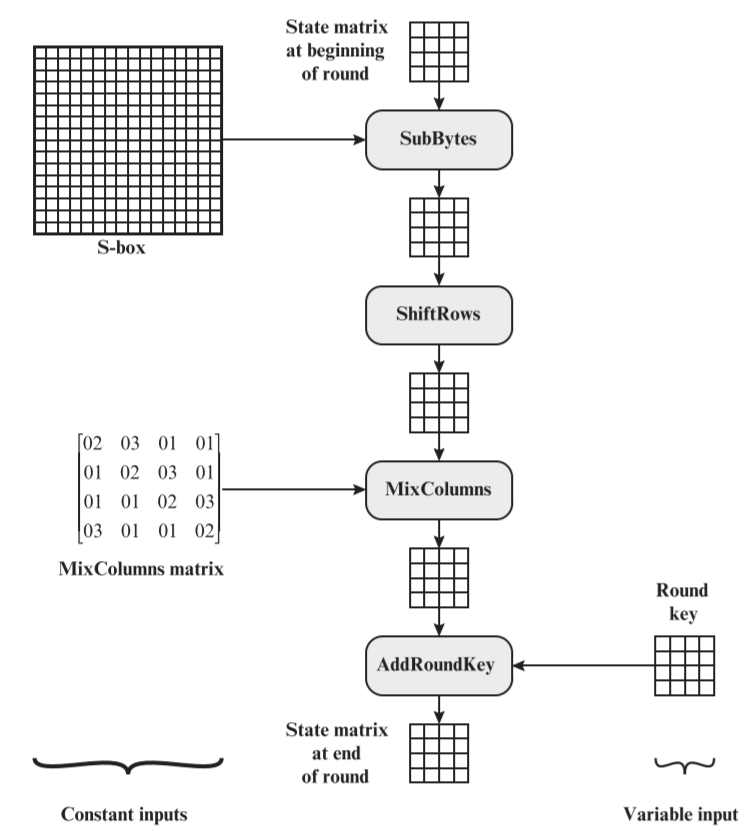
\includegraphics[width=3.0in]{fig/singleround.png}
\end{frame}

\begin{frame}{Key Expansion}
	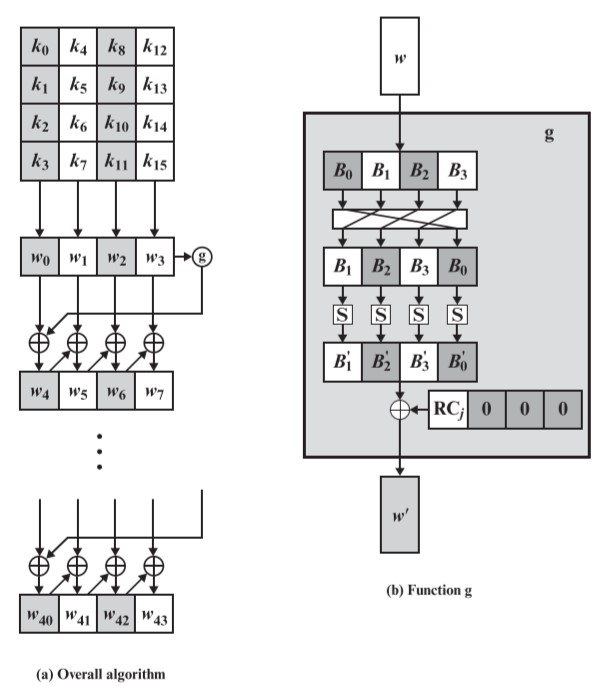
\includegraphics[width=2.8in]{fig/clip_image020.jpg}
\end{frame}

\begin{frame}{Decryption}
	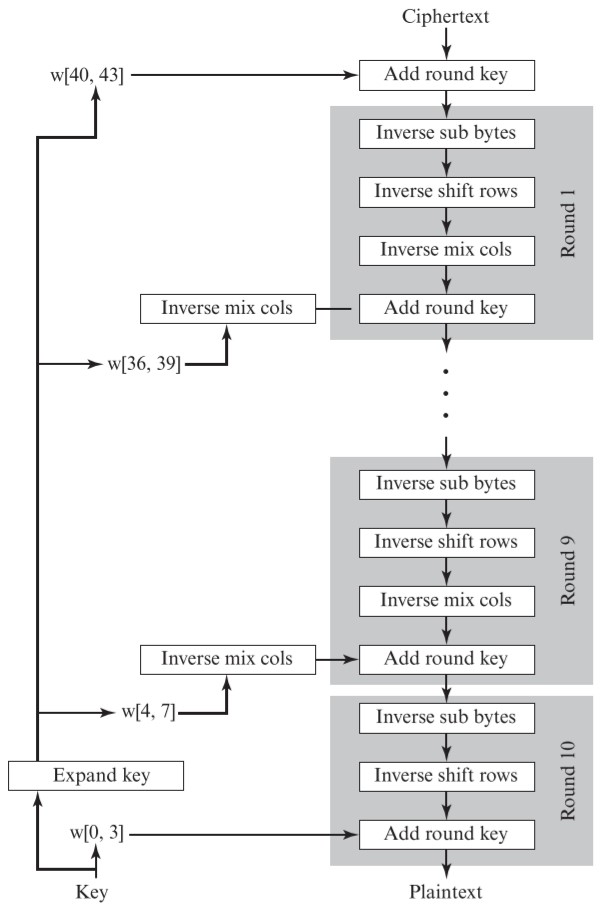
\includegraphics[width=2.1in]{fig/clip_image022.jpg}

\end{frame}

\begin{frame}{Note}
	The S-box and the inverse S-box are the only two nonlinear operations
	within the Advanced Encryption Standard.
\end{frame}

\begin{frame}
	\centering \Large
	\emph{Thanks}
\end{frame}

\end{document}
